\subsection{Eingabeknoten}

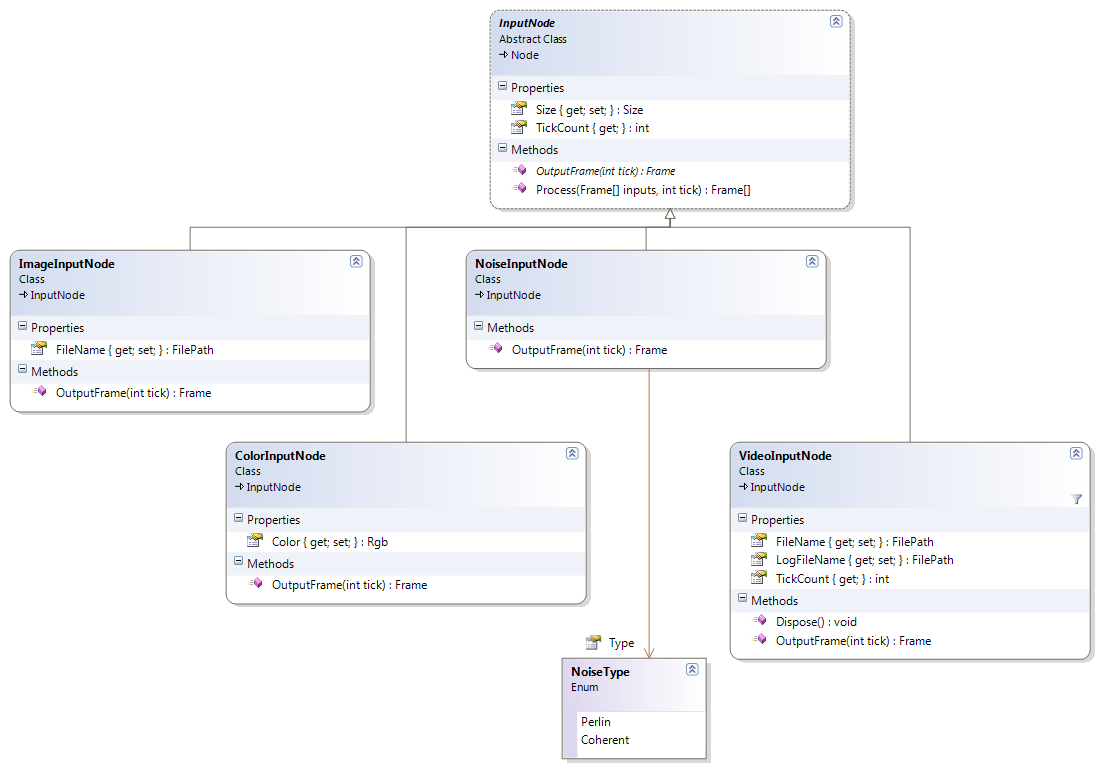
\includegraphics[width=\textwidth]{YuvKA.Pipeline/inputnodes.png}
Der im Folgenden spezifizierte Teil des Programmes beschreibt die Knoten, welche die Eingabedaten der Pipeline bereitstellen. Alle solchen Knoten erben von der abstrakten Klasse \name{InputNode}, welche die Member \name{TickCount} und \name{Size} definiert, die die Anzahl an zu liefernden \name{Frame}s bzw. die Größe eines jeden \name{Frame}s angeben.
\name{InputNode} selbst erbt von der \name{Node}-Klasse.


\subsubsection{YuvKA.Pipeline.InputNode}

\begin{verbatim}
[DataContract]
public abstract class InputNode : Node
\end{verbatim}

\paragraph{Beschreibung}~\\
Die abstrakte Klasse \name{InputNode} modelliert die Eingabequellen der Pipeline und liefert eine gemeinsame Basis für deren konkrete Implementierungen.

\paragraph{Typmember}
\begin{itemize}

\property{Size}
	\begin{verbatim}
	[DataMember]
	public Size Size { get; set; }
	\end{verbatim}
	Spezifiziert die Größe des vom Knoten gelieferten \name{Frame}s in Form eines \name{Size}-Objektes.

\property{TickCount}
	\begin{verbatim}
	[Browsable(false)]
	public virtual int TickCount { get; }
	\end{verbatim}
	Ruft die Anzahl an vom Knoten zu liefernden \name{Frame}s ab. Der Standardrückgabewert ist 1, die Methode ist allerdings in Unterklassen überschreibbar.

\end{itemize}

\subsubsection{YuvKA.Pipeline.ImageInputNode}

\begin{verbatim}
[DataContract]
public class ImageInputNode : InputNode
\end{verbatim}

\paragraph{Beschreibung}~\\
Die Klasse \name{ImageInputNode} stellt die Funktionalität eines Knotens dar, der lediglich ein aus einer Datei im PNG-Format gelesenes Standbild in die Pipeline einspeist. Sie erbt von der abstrakten \name{InputNode}-Klasse.

\paragraph{Typmember}
\begin{itemize}

\property{FileName}
	\begin{verbatim}
[DisplayName("File Name")]
[DataMember]
public FilePath FileName { get; set; }
	\end{verbatim}
	Entspricht dem Dateipfad der zu benutzenden Datei.

\method{Process}
	\begin{verbatim}
	public override Frame[] Process(Frame[] inputs, int tick)
	\end{verbatim}
	Ignoriert den Wert der Eingabeparameter und liefert als Rückgabewert ein Array der Größe 1, das einen \name{Frame} mit den Bilddaten der Datei (aus dem Pfad \name{FileName}) enthält.

\end{itemize}
\subsubsection{YuvKA.Pipeline.ColorInputNode}

\begin{verbatim}
[DataContract]
public class ColorInputNode : InputNode
\end{verbatim}

\paragraph{Beschreibung}~\\
Die Klasse \name{ColorInputNode} liefert die Funktionalität, einen Videostream einer benutzerdefinierten Farbe in Form von \name{Frame}s an die Pipeline zu liefern. Sie erbt von der abstrakten \name{InputNode}-Klasse.

\paragraph{Typmember}
\begin{itemize}

\property{Color}
	\begin{verbatim}
	[DataMember]
	public Rgb Color { get; set; }
	\end{verbatim}
	Entspricht der als Quellwert benutzten Farbe.


\method{Process}
	\begin{verbatim}
	public override Frame[] Process(Frame[] inputs, int tick)
	\end{verbatim}
	Ignoriert den Wert der Eingabeparameter und liefert als Rückgabewert ein Array der Größe 1, das einen \name{Frame} enthält welcher vollends mit der vom Benutzer gewählten Farbe ausgefüllt ist.

\end{itemize}

\subsubsection{YuvKA.Pipeline.NoiseInputNode}

\begin{verbatim}
[DataContract]
public class NoiseInputNode : InputNode
\end{verbatim}

\paragraph{Beschreibung}~\\
Die Klasse \name{NoiseInputNode} stellt einen Knoten bereit, welcher eine von zwei Arten zufällig generierter Videostreams in Form von \name{Frame}s mit Rauschsignal an die Pipeline liefert. Die Klasse erbt von der abstrakten \name{InputNode}-Klasse.

\paragraph{Typmember}
\begin{itemize}

\property{Type}
	\begin{verbatim}
	[DataMember]
	public NoiseType Type { get; set; }
	\end{verbatim}
	Setzt den Typ des Videostreams fest, welcher generiert wird. Standardmäßig werden folgende Verfahren unterstützt:
	\begin{description}
		\item[Perlin-Noise]~\\
		Bei Perlin-Noise werden pseudozufällige Signale dadurch generiert, dass die Koordinaten des angefragten Punktes anhand eines vorgerechneten Rasters mit zufälligen Vektoren nachgeschlagen werden. Der resultierende Wert ist das Resultat des Skalarproduktes aus Abstandsvektors (zum nächsten Rasterpunkt) mit dem im Raster gefundenen Vektor, kombiniert mit einfacher Interpolation, um das resultierende Bild stetig zu halten. PseudoCode der 2-dimensionalen Version:
\begin{verbatim}
public double PerlinNoise(int x, int y) {
  int xint = Math.floor(x);
  int yint = Math.floor(y);
  // Vorberechnete Vektoren an nächsten Gitterpunkten
  // Nachschlagen und das Skalarprodukt mit dem 
  // Abstandsvektor zu den Koordinaten bilden
  latticeVect0 = DotProduct(randVectors[xint, yint],
                            (x - xint, y - yint) );
  latticeVect1 = DotProduct(randVectors[xint+1, yint], 
                            (x - xint-1, y - yint) );
  latticeVect2 = DotProduct(randVectors[xint, yint+1], 
                            (x - xint, y - yint-1) );
  latticeVect3 = DotProduct(randVectors[xint+1, yint+1], 
                            (x - xint-1, y - yint-1) );

  // Resultate interpolieren
  xValue = interpolate(latticeVect0, latticeVect1);
  yValue = interpolate(latticeVect2, latticeVect3);
  return interpolate(xValue, yValue);
\end{verbatim}
        Das Resultat von diesem Algorithmus muss bei der weiteren Verarbeitung noch an den Farbraum (hier RGB) angepasst werden. Anzumerken ist, dass es sich hierbei um die ``Rohform'' des Algorithmus handelt, bei der nur eine Iteration durchgeführt wird.
		\item[Coherent Noise]~\\
		Hierbei handelt es sich um einfaches, kohärentes Bildrauschen, welches pixelweise erzeugt wird.
	\end{description}

\method{Process}
	\begin{verbatim}
	public override Frame[] Process(Frame[] inputs, int tick)
	\end{verbatim}
	Ignoriert den Wert der Eingabeparameter und liefert als Rückgabewert ein Array der Größe 1, das den generierten \name{Frame} enthält. Das benutzte Generierungsverfahren hängt vom Wert von \name{Type} ab.


\end{itemize}

\subsubsection{YuvKA.Pipeline.VideoInputNode}

\begin{verbatim}
[DataContract]
public class VideoInputNode : InputNode
\end{verbatim}

\paragraph{Beschreibung}~\\
Die Klasse \name{VideoInputNode} modelliert einen Knoten, welcher die Daten eines aus einer Datei gelesenen Videostream in die Pipeline einspeist. Befindet sich an der durch \name{LogFileName} angegebenen Stelle eine gültige Log-Datei, so wird diese als Metadaten mit einem \name{AnnotatedFrame} mitgereicht. Sie erbt von der abstrakten \name{InputNode}-Klasse.


\paragraph{Typmember}
\begin{itemize}

\property{FileName}
        \begin{verbatim}
[DisplayName("Video File")]
[DataMember]
public FilePath FileName { get; set; }
        \end{verbatim}
	Ruft den Dateipfad der zu lesenden Videodatei ab oder setzt diesen fest.

\property{LogFileName}
        \begin{verbatim}
[DisplayName("Optional Log File")]
[DataMember]
public FilePath LogFileName { get; set; }
        \end{verbatim}
	Ruft den Dateipfad der (optionalen) zu lesenden Log-Datei ab oder setzt diesen fest.

\property{TickCount}
        \begin{verbatim}
[Browsable(false)]
public override int TickCount { get; }
        \end{verbatim}
	Ruft die Anzahl der im Videostream befindlichen \name{Frame}s ab.

\method{Dispose}
        \begin{verbatim}
public override void Dispose()
        \end{verbatim}
Schließt den Videostream, sodass das File-Handle freigegeben wird.


\end{itemize}
